\documentclass[conference,a4paper]{IEEEtran}
\IEEEoverridecommandlockouts

\usepackage[T1]{fontenc}
\usepackage{cite}
\usepackage{amsmath,amssymb,amsfonts}
\usepackage{algorithmic}
\usepackage{graphicx}
\usepackage{textcomp}
\usepackage{xcolor}
\usepackage{microtype}
\usepackage{array}
\usepackage{booktabs}
\usepackage{placeins}
\usepackage{fancyhdr}
\newcolumntype{L}[1]{>{\raggedright\arraybackslash}p{#1}}
\newcolumntype{C}[1]{>{\centering\arraybackslash}p{#1}}
\emergencystretch=2em

\def\BibTeX{{\rm B\kern-.05em{\sc i\kern-.025em b}\kern-.08em
    T\kern-.1667em\lower.7ex\hbox{E}\kern-.125emX}}

% Navigation bookmarks: gives the PDF an outline pane in Acrobat, Edge,
% Okular, VS Code's viewer, etc. hidelinks keeps the printed page identical
% (no coloured or boxed links), so this changes navigation only, not layout.
% hyperref is loaded last, as it must be.
\usepackage[hidelinks,bookmarks=true,bookmarksnumbered=true,
            bookmarksopen=true,bookmarksopenlevel=2,
            pdftitle={How Much Does the Activation Function Matter?
                      A 2000-Run Variance Study of Gated Recurrent Networks
                      for Sentiment Classification},
            pdfsubject={iCONEECT 2026}]{hyperref}

% ── iCONEECT 2026 camera-ready: first-page header and copyright footer ─────
% Both are required on page 1 only. \fancyhf{} clears IEEEtran's own footer,
% so the copyright notice is printed here rather than left to \IEEEpubid;
% \IEEEpubid is still issued after \maketitle so IEEEtran reserves the
% column space and body text cannot collide with the notice.
\fancypagestyle{firstpage}{%
  \fancyhf{}%
  \renewcommand{\headrulewidth}{0pt}%
  \renewcommand{\footrulewidth}{0pt}%
  \fancyhead[L]{\fontsize{9}{10}\selectfont
    \parbox{\textwidth}{2026 1st International Conference on Next-Generation
    Electrical \& Electronics, Computer Systems, and Technologies (iCONEECT).\\
    25--26 September, 2026, Premier University, Chittagong, Bangladesh}}%
  \fancyfoot[L]{\fontsize{9}{10}\selectfont
    979-8-3195-4810-8/26/\$31.00~\copyright2026 IEEE}%
}

\title{How Much Does the Activation Function Matter?\\
A 2{,}000-Run Variance Study of Gated Recurrent\\
Networks for Sentiment Classification}

\author{%
\IEEEauthorblockN{[AUTHOR 1 NAME]}
\IEEEauthorblockA{\textit{[DEPT 1]} \\
\textit{[INSTITUTION 1]}\\{}
[CITY 1], [COUNTRY 1] \\{}
[EMAIL 1]}
\and
\IEEEauthorblockN{[AUTHOR 2 NAME]}
\IEEEauthorblockA{\textit{[DEPT 2]} \\
\textit{[INSTITUTION 2]}\\{}
[CITY 2], [COUNTRY 2] \\{}
[EMAIL 2]}
\and
\IEEEauthorblockN{[AUTHOR 3 NAME]}
\IEEEauthorblockA{\textit{[DEPT 3]} \\
\textit{[INSTITUTION 3]}\\{}
[CITY 3], [COUNTRY 3] \\{}
[EMAIL 3]}
}

\begin{document}
\raggedbottom

% iCONEECT 2026 camera-ready: first-page footer (copyright notice).
% \IEEEpubid must follow \maketitle to take effect on page 1.
\IEEEpubid{\makebox[\columnwidth]{979-8-3195-4810-8/26/\$31.00~\copyright2026
  IEEE\hfill}\hspace{\columnsep}\makebox[\columnwidth]{}}

\maketitle
\thispagestyle{firstpage}
\IEEEpubidadjcol

\begin{abstract}
Activation-function comparisons in gated recurrent networks are
almost always reported from a single training run. It has therefore
never been established whether the differences they report are
larger than the noise of retraining the same model. This paper
settles that question at scale. We train all 100 ordered pairs of ten
activation functions in the dense layers of four gated recurrent
architectures on IMDb, and repeat every one of the 400
configurations under five random seeds, for \textbf{2{,}000 models}
in total with every other setting held fixed. A variance
decomposition over these runs shows that the random seed accounts
for \textbf{58.7\%} of all variation in test accuracy and the
architecture for \textbf{26.7\%}, while the activation pair explains
only \textbf{3.7\%}. The consequence is direct: single-seed
activation rankings do not reproduce. Across the four
architectures the Spearman correlation between the single-seed
ranking of the 100 pairs and their five-seed means is
$-0.174$, $-0.059$, $-0.041$ and $+0.055$, indistinguishable from
zero in every case, and the ten best configurations overlap within
their confidence intervals. What survives is architectural: GRU
outperforms LSTM by 0.79 points ($p<10^{-100}$, Cohen's $d=1.19$),
supplies all fifty highest-scoring configurations, and is the more
reliable choice, with roughly 40\% lower seed-to-seed standard
deviation. One activation effect also survives: smooth
functions reach 73.7\% validation accuracy after one epoch against
61.1\% for the ReLU family. These results support reporting both
mean accuracy and variation across training seeds in activation
comparisons.
\end{abstract}

\begin{IEEEkeywords}
Sentiment Analysis, IMDb Dataset, Deep Learning, LSTM, GRU, Activation Functions, Reproducibility, Seed Variance, Experimental Methodology.
\end{IEEEkeywords}

\section{Introduction}

Sentiment analysis is the task of deciding whether a piece of
text is positive or negative. It is one of the most common
problems in natural language processing. The IMDb Large
Movie Review Dataset, with 50{,}000 balanced reviews, is the
standard benchmark for the binary version of the
task~\cite{maas2011}. LSTM and GRU networks are the usual
choice for this problem because their gating mechanisms let
them track context across long sequences~\cite{hochreiter1997,cho2014,chung2014}.

One part of these models gets little attention: the activation
function in the dense layers that sit after the recurrent
layers. The gates inside the recurrent cell are fixed to
sigmoid and tanh, but the dense layers that turn the recurrent
output into a final prediction can use any activation function.
Ahmed et al.~\cite{ahmed2025} tested three classical
combinations in a bidirectional LSTM, reached 88.40\% accuracy,
and asked for follow-up work on modern activation functions and
other architectures.

Interpreting activation comparisons
\cite{eger2018,farzad2019,essaiAli2022,zhu2022,ahmed2025}
requires separating differences between functions from variation
between training runs. Weight initialisation, dropout masks and
batch order can change accuracy even when the data and training
settings stay fixed. A high score from one run therefore provides
limited evidence for preferring one activation function.

We evaluate all 100 ordered pairs of ten activation functions
in two dense layers across four LSTM/GRU architectures. Training
each of the 400 configurations with five seeds gives
\textbf{2{,}000 runs} on a fixed data split. We compare mean
accuracy, consistency across seeds and ranking agreement;
a separate follow-up examines early learning. We address six
questions:

\begin{itemize}\itemsep0pt
  \item \textbf{RQ1:} How much accuracy variation comes from
        architecture, activation choice and training seeds?
  \item \textbf{RQ2:} Which architectures achieve higher mean
        test accuracy?
  \item \textbf{RQ3:} How do accuracy gaps between leading
        activation pairs compare with variation across seeds?
  \item \textbf{RQ4:} Do single-run rankings agree with
        five-seed rankings?
  \item \textbf{RQ5:} How does activation choice affect early
        learning?
  \item \textbf{RQ6:} Which architectures give more consistent
        test accuracy across training runs?
\end{itemize}

\FloatBarrier
\section{Literature Review}

Hochreiter and Schmidhuber~\cite{hochreiter1997} introduced
the LSTM to address the vanishing gradient problem in
recurrent networks, using sigmoid and tanh within the
recurrent cell. Cho et al.~\cite{cho2014} proposed the GRU,
which uses two gates and combines the cell and hidden
states. Chung et al.~\cite{chung2014} compared GRU and LSTM
on sequence-modeling tasks and found GRU competitive with
LSTM. Schuster and Paliwal~\cite{schuster1997} introduced
bidirectional recurrent networks, allowing models to use
both past and future context. These studies established
the recurrent architectures used in our comparison.

The activation function literature developed alongside
these architectural advances. Nair and Hinton~\cite{nair2010}
studied ReLU, which avoids saturation for positive inputs
but has zero gradients for negative inputs. Maas et
al.~\cite{maas2013} and Clevert et al.~\cite{clevert2015}
studied LeakyReLU and ELU, which allow nonzero outputs for
negative inputs. Klambauer et al.~\cite{klambauer2017}
introduced SELU with self-normalising properties under
specific conditions. Later work introduced
GELU~\cite{hendrycks2016}, Swish~\cite{ramachandran2017},
and Mish~\cite{misra2020}, while
surveys~\cite{nwankpa2018,apicella2021} reviewed the growing
range of activation functions. These developments motivate
examining their effects in the dense layers following
gated recurrent networks.

Within sentiment analysis, IMDb~\cite{maas2011} is a widely
used binary classification benchmark. Tang et
al.~\cite{tang2015} studied gated recurrent networks for
document-level sentiment classification, and Socher et
al.~\cite{socher2013} introduced the Stanford Sentiment
Treebank. Several studies have examined activation choice.
Eger et al.~\cite{eger2018} compared 21 activations across
eight NLP tasks and also investigated alternative
activations within LSTM cells. Farzad et
al.~\cite{farzad2019} compared 23 activation functions in
a basic LSTM network on IMDb, Movie Review, and MNIST.
Essai Ali et al.~\cite{essaiAli2022} evaluated 26 state
activation functions in LSTM networks on classification
tasks outside sentiment analysis. Zhu and
Tan~\cite{zhu2022} tested a custom activation in simple RNN,
LSTM, and GRU models on IMDb, comparing it with ReLU,
LeakyReLU, ELU, SELU, and tanh. Ahmed et
al.~\cite{ahmed2025} compared three classical activation
pairings in a bidirectional LSTM, reported 88.40\% accuracy,
and suggested examining modern functions and other
architectures.

Our study brings these comparisons into a shared experimental
design. We evaluate all 100 ordered pairs of ten activation
functions in two dense layers across four architectures.
These use LSTM or GRU cells, a bidirectional first recurrent
layer, and either a unidirectional or bidirectional second
layer. The comparison includes GELU, SiLU, and Mish, with
the data split and training settings held fixed.

Repeated training is also part of earlier work. Eger et
al.~\cite{eger2018} explicitly averaged results over five
random weight initializations in their sentence-classification
experiments. Our main contribution is therefore the analysis
of how variation between training runs compares with the
effects of architecture and dense-layer activation choice
in this setting. We train every configuration with five
seeds and examine whether rankings from one run agree with
rankings based on repeated runs. This allows us to assess
which performance differences are clear and which remain
uncertain.%heyyy
\FloatBarrier
\section{Methodology}
%------------------------------------------------------------------------------
\subsection{Dataset and Preprocessing}

The IMDb Large Movie Review Dataset~\cite{maas2011} (50,000
reviews, balanced binary labels) was split 80/20 train-test
with \texttt{random\_state=42}, and 10\% of
training data was withheld as a validation set. Reviews were
cleaned by removing HTML tags and non-alphabetic characters,
then lowercased. A vocabulary of the 5,000 most frequent
training-set tokens was used; all sequences were truncated or
zero-padded to 200 tokens (Table~\ref{tab:hyperparams}).

\subsection{Network Architecture}

All four experiments share the same model structure. The
only thing that changes within each experiment is the choice of
Act$_1$ and Act$_2$ in the two dense layers. The shared architecture
is: an embedding layer
(vocabulary 5,000, dimension 128), a bidirectional recurrent
Layer~1 (64 units per direction), a recurrent Layer~2 (32
units per direction), Dropout(0.4), Dense Layer~1 (64 units)
with Act$_1$, Dense Layer~2 (32 units) with Act$_2$, and a
single output unit trained with \texttt{BCEWithLogitsLoss}.
The four experiments differ only in the recurrent cell type
(LSTM, GRU) and whether Layer 2
is bidirectional (Table~\ref{tab:architectures}).

\begin{table}[htbp]
  \caption{Experimental Architecture Summary}
  \label{tab:architectures}
  \centering
  \footnotesize
  \setlength{\tabcolsep}{4pt}
  \renewcommand{\arraystretch}{1.08}
  \begin{tabular}{cllr}
    \toprule
    Exp. & Layer 1 & Layer 2 & Params \\
    \midrule
    1 & BiLSTM(64) & LSTM(32)    & ${\approx}$764K \\
    2 & BiGRU(64)  & GRU(32)     & ${\approx}$734K \\
    3 & BiLSTM(64) & BiLSTM(32)  & ${\approx}$787K \\
    4 & BiGRU(64)  & BiGRU(32)   & ${\approx}$752K \\
    \bottomrule
  \end{tabular}
\end{table}

\subsection{Activation Functions Under Investigation}

Ten activation functions were evaluated
(Table~\ref{tab:activations}). The classical family is
ReLU~\cite{nair2010}, LeakyReLU~\cite{maas2013},
PReLU~\cite{he2015}, ELU~\cite{clevert2015}, Tanh and
SELU~\cite{klambauer2017}. The modern smooth family is
GELU~\cite{hendrycks2016}, SiLU (Swish)~\cite{ramachandran2017},
Mish~\cite{misra2020} and Hardswish~\cite{howard2019}. The latter
four had not previously been benchmarked in gated recurrent dense
layers for sentiment classification.

\begin{table}[htbp]
  \caption{Activation Functions: Families and Key Properties}
  \label{tab:activations}
  \centering\footnotesize
  \setlength{\tabcolsep}{3pt}
  \renewcommand{\arraystretch}{1.05}
  \resizebox{\columnwidth}{!}{%
  \begin{tabular}{lll}
    \toprule
    Function & Type & Formula / Key Property \\
    \midrule
    ReLU      & Classical & $\max(0,x)$; dead neurons for $x{<}0$ \\
    ELU       & Classical & $\alpha(e^x{-}1)$ for $x{\leq}0$; mean-centering \\
    LeakyReLU & Classical & $0.01x$ for $x{<}0$; low dead-neuron risk \\
    Tanh      & Classical & Bounded; saturates for $|x|\gg1$ \\
    GELU      & Modern & $x\cdot\Phi(x)$; probabilistic gating \\
    SiLU      & Modern & $x\cdot\sigma(x)$; self-gating \\
    Mish      & Modern & $x\cdot\tanh(\text{softplus}(x))$; smooth \\
    SELU      & Modern & Self-normalising; implicit batch norm \\
    PReLU     & Modern & Learnable slope $a$; input-dependent \\
    Hardswish & Modern & Piecewise; dead zone for $x{<}{-3}$ \\
    \bottomrule
  \end{tabular}%
  }
\end{table}

\subsection{Training Configuration and Evaluation}

Every setting in Table~\ref{tab:hyperparams} was held the
same across all runs, so the activation pair is the only
thing that changes between models. The architecture parameters
(vocabulary, embedding, layer sizes, dropout) replicate
Ahmed et al.~\cite{ahmed2025} exactly. The training parameters
(optimizer, learning rate, batch size, scheduler, clipping)
were chosen by us because Ahmed et al. did not report them.
After training, accuracy, precision, recall, and F1-score were
measured on the held-out 10,000-review test set.

\subsection{Replication Protocol}
\label{sec:replication}

Each of the $10\times10\times4 = 400$ configurations was trained
under five seeds, $\{10,20,30,40,50\}$
(Table~\ref{tab:hyperparams}), giving $2{,}000$ models.
The seed is applied immediately before the model and its data
loaders are constructed, setting \texttt{random}, \texttt{numpy},
\texttt{torch} and \texttt{torch.cuda} with
\texttt{cudnn.deterministic=True}, so a given (pair, seed) is
exactly reproducible.

The split is deliberately \emph{not} a function of the seed: it
stays pinned at \texttt{random\_state=42}. The variance we report
is therefore the variance of retraining the same model on the same
data. That is the quantity a single-run comparison assumes to be
negligible. Split variance would only inflate it, so these
estimates are conservative.

Runs were executed five at a time, one worker per seed. Each
worker is a separate process with its own RNG and deterministic
kernel selection, so concurrency cannot perturb a result; we
confirmed this by re-running sampled configurations serially and
recovering identical metrics.

\begin{table}[htbp]
  \caption{Shared Hyperparameter Configuration}
  \label{tab:hyperparams}
  \centering\footnotesize
  \setlength{\tabcolsep}{3pt}
  \renewcommand{\arraystretch}{1.05}
  \resizebox{\columnwidth}{!}{%
  \begin{tabular}{lll}
    \toprule
    Hyperparameter & Value & Source \\
    \midrule
    Vocab / Seq.\ length / Embed. & 5{,}000 / 200 / 128 & \cite{ahmed2025} \\
    RNN Layer 1 / Layer 2 units   & 64 / 32 per direction & \cite{ahmed2025} \\
    Dense Layer 1 / Layer 2 units & 64 / 32 & \cite{ahmed2025} \\
    Dropout rate                  & 0.4 & \cite{ahmed2025} \\
    Batch size / Max epochs       & 64 / 10 & Ours \\
    Early stopping patience       & 3 epochs (val.\ loss) & Ours \\
    Optimiser                     & Adam, $\text{lr}=10^{-3}$ & Ours \\
    LR scheduler                  & ReduceLROnPlateau ($\times$0.5) & Ours \\
    Loss / Gradient clipping      & BCEWithLogitsLoss / $L_2\leq1.0$ & Ours \\
    Weight initialisation         & Kaiming uniform (Linear) & PyTorch default \\
    Data split seed               & 42, fixed for all runs & Ours \\
    Training seeds                & 10, 20, 30, 40, 50 & Ours \\
    \bottomrule
  \end{tabular}%
  }
\end{table}

\subsection{On Reproducing the Baseline of Ahmed et al.}
\label{sec:baseline_repro}

Ahmed et al.~\cite{ahmed2025} describe their architecture in full
and we copy it exactly, but they do not report how they trained
it: optimizer, learning rate, batch size, epochs, early stopping,
seed and data split are all missing. Exact reproduction is
therefore impossible, and we adopt the fully documented settings of
Table~\ref{tab:hyperparams} instead.

Replication sharpens what can be said about their 88.40\%. Our best
configuration averages 87.81\% (Table~\ref{tab:top_configs})
with a 95\% upper bound of 88.01\%,
and no run among the 2{,}000 reached 88.40\% (maximum 88.39\%), so
the benchmark sits outside the interval of our strongest setting.
Since they report a single run without a seed or standard
deviation, and we measure the per-cell standard deviation of this
model family at 0.38 points, their figure is best read as one draw
of unknown uncertainty. We treat it as a reference point, not a
target.
%------------------------------------------------------------------------------
\FloatBarrier\section{Results}
\label{sec:results}

\subsection{Variation in Test Accuracy}
\label{sec:variance}

Variation across the five seeds within each configuration
accounts for \textbf{58.7\%} of total test-accuracy variance,
the largest component (Table~\ref{tab:variance}). Architecture
accounts for 26.7\%, and activation pairs for 3.7\%. Seed
variation is therefore about sixteen times the activation-pair
component. A further 10.9\% comes from the architecture--activation
interaction: differences between activation pairs change
across architectures.

Within the architecture component, the choice between LSTM
and GRU accounts for 26.3\% of total variance, compared with
0.19\% for making the second recurrent layer bidirectional.

\begin{table}[htbp]
  \caption{Sources of Variation in Test Accuracy (2{,}000 Runs)}
  \label{tab:variance}
  \centering\footnotesize
  \setlength{\tabcolsep}{4pt}
  \renewcommand{\arraystretch}{1.08}
  \begin{tabular}{@{}lr@{}}
    \toprule
    Source of variation & \% of total variance \\
    \midrule
    Architecture (4 types) & 26.69 \\
    Activation pair (100 pairs) & 3.74 \\
    Architecture--activation interaction & 10.90 \\
    Training seed (within configuration) & 58.67 \\
    \midrule
    \textbf{Total} & \textbf{100.00} \\
    \bottomrule
  \end{tabular}

  \vspace{4pt}
  \parbox{\columnwidth}{\scriptsize
    Each configuration uses one architecture and one activation
    pair. Seed variation is measured across its five training
    runs. The interaction measures how differences between
    activation pairs change across architectures.
  }
\end{table}

\subsection{Classification Performance}
\label{sec:classification}
\begin{table}[htbp]
  \caption{Cross-Experiment Accuracy over 2{,}000 Runs (500 per Experiment)}
  \label{tab:sweep_summary}
  \centering\footnotesize
  \setlength{\tabcolsep}{3pt}
  \renewcommand{\arraystretch}{1.1}
  \resizebox{\columnwidth}{!}{%
  \begin{tabular}{lccccc}
    \toprule
    Experiment & Min\% & Max\% & Mean\% & 95\% CI & $\sigma_{\text{cell}}$ \\
    \midrule
    BiLSTM+LSTM & 82.06 & 87.16 & \textbf{86.62} & $\pm$0.10 & 0.53 \\
    BiGRU+GRU & 87.12 & 87.81 & \textbf{87.48} & $\pm$0.03 & 0.33 \\
    BiLSTM+BiLSTM & 86.07 & 87.14 & \textbf{86.75} & $\pm$0.05 & 0.48 \\
    BiGRU+BiGRU & 87.14 & 87.73 & \textbf{87.48} & $\pm$0.03 & 0.29 \\
    \midrule
    \multicolumn{3}{l}{\textbf{Benchmark}~\cite{ahmed2025}} & \textbf{88.40} & --- & --- \\
    \bottomrule
    \multicolumn{6}{l}{\small Min/Max are over the 100 cell means; $\sigma_{\text{cell}}$ is the median} \\
    \multicolumn{6}{l}{\small per-cell standard deviation across the five seeds.} \\
  \end{tabular}%
  }
\end{table}


Both GRU architectures have higher mean accuracy than both
LSTM architectures (Table~\ref{tab:sweep_summary}). Each
architecture mean covers 500 runs: 100 activation pairs
trained with five seeds each. Both GRU means round to
87.48\%, compared with 86.62\% for BiLSTM+LSTM and 86.75\%
for BiLSTM+BiLSTM. Across 1{,}000 runs per family, GRU
averages 87.48\% and LSTM 86.69\%, a gap of
\textbf{0.79 percentage points}.

Table~\ref{tab:sweep_summary} also reports the median standard
deviation (SD) across the five seeds for each architecture's
100 configurations. These SDs describe consistency for a fixed
activation pair; the spread of points in
Fig.~\ref{fig:architecture_spread} instead shows differences
between the pairs' five-seed means.

\begin{figure}[htbp]
  \centering
  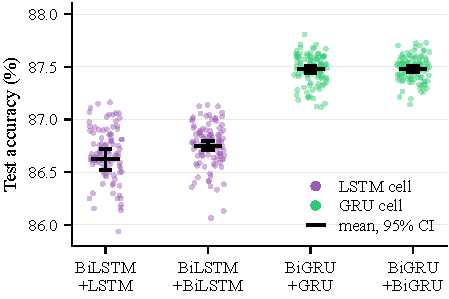
\includegraphics[width=0.92\columnwidth]{assets/architecture_spread.pdf}
  \caption{Each point is an activation pair's mean test accuracy
  over five seeds. Each architecture has 100 pairs; black
  horizontal markers show architecture means. The plot shows
  99 points for BiLSTM+LSTM and 100 for each other architecture.
  Hardswish + LeakyReLU in BiLSTM+LSTM falls below the 85.8\%
  axis limit (mean 82.06\%, SD 9.27 percentage points).}
  \label{fig:architecture_spread}
\end{figure}

\subsection{The Ten Highest Mean Accuracies}

All ten leading configurations use GRU, as do the top fifty
of the 400 tested configurations. ReLU + LeakyReLU in
BiGRU+GRU has the highest five-seed mean at 87.81\%, with
an SD of 0.17 percentage points (Table~\ref{tab:top_configs}).
The highest individual accuracy among all 2{,}000 runs is
88.39\%.

The ten means range from 87.68\% to 87.81\%, spanning
0.124 percentage points before rounding. Their seed SDs
range from 0.10 to 0.40 points. For nine of the ten
configurations, the SD exceeds the entire span of the ten
means. Variation between runs therefore often exceeds the mean
gaps; this comparison alone does not establish statistical
significance.

\begin{table}[htbp]
  \caption{Ten Highest-Accuracy Configurations of 400, with Seed Variability}
  \label{tab:top_configs}
  \centering\footnotesize
  \renewcommand{\arraystretch}{1.1}
  \resizebox{\columnwidth}{!}{%
  \begin{tabular}{llccc}
    \toprule
    Act$_1$ + Act$_2$ & Experiment & Acc.\% & 95\% CI & F1\% \\
     &  & mean $\pm$ $\sigma$ & $\pm$ & mean \\
    \midrule
    ReLU + LeakyReLU & BiGRU+GRU & 87.81 $\pm$ 0.17 & 0.21 & 87.80 \\
    SiLU + Mish & BiGRU+BiGRU & 87.73 $\pm$ 0.16 & 0.20 & 87.65 \\
    Tanh + LeakyReLU & BiGRU+BiGRU & 87.72 $\pm$ 0.40 & 0.50 & 87.70 \\
    Tanh + GELU & BiGRU+GRU & 87.71 $\pm$ 0.29 & 0.36 & 87.75 \\
    PReLU + ReLU & BiGRU+GRU & 87.71 $\pm$ 0.17 & 0.22 & 87.67 \\
    GELU + GELU & BiGRU+BiGRU & 87.70 $\pm$ 0.18 & 0.22 & 87.58 \\
    SiLU + Hardswish & BiGRU+BiGRU & 87.70 $\pm$ 0.10 & 0.12 & 87.69 \\
    GELU + Hardswish & BiGRU+BiGRU & 87.69 $\pm$ 0.18 & 0.23 & 87.65 \\
    SiLU + GELU & BiGRU+GRU & 87.68 $\pm$ 0.18 & 0.22 & 87.63 \\
    PReLU + GELU & BiGRU+GRU & 87.68 $\pm$ 0.28 & 0.34 & 87.71 \\
    \bottomrule
    \multicolumn{5}{l}{\small All ten are GRU-based. The ten means span 0.12 points, less than} \\
    \multicolumn{5}{l}{\small the widest half-interval ($\pm$0.50); every pair of intervals overlaps.} \\
  \end{tabular}%
  }
\end{table}


\subsection{Agreement Between Single-Seed and Five-Seed Rankings}

Within each architecture, we ranked the 100 activation pairs
by their original single-run accuracy and by their five-seed
mean. All four original winners rank 77th or lower by five-seed mean.
Table~\ref{tab:original_winners} compares their original
accuracies with their repeated-run means.

\input{tables/tab8_original_winners.tex}

Across all 100 pairs, Spearman rank correlations range from
$-0.174$ to $+0.055$, indicating little agreement
(Table~\ref{tab:reproducibility}). Pairs move an average of
32.1--36.9 places, and each architecture's two top-ten lists
have at most one pair in common. The mean absolute difference
between original accuracy and five-seed mean is 0.34--0.53
percentage points.

\begin{table}[htbp]
  \caption{Agreement Between the Single-Seed Ranking and the 5-Seed Means}
  \label{tab:reproducibility}
  \centering\footnotesize
  \setlength{\tabcolsep}{3pt}
  \renewcommand{\arraystretch}{1.1}
  \resizebox{\columnwidth}{!}{%
  \begin{tabular}{lcccc}
    \toprule
    Experiment & $\rho$ & Mean rank $\Delta$ & Top-10 overlap & Mean $|\Delta$acc$|$ \\
    \midrule
    BiLSTM+LSTM & $-0.174$ & 36.9 & 0/10 & 0.53 \\
    BiGRU+GRU & $-0.059$ & 34.5 & 1/10 & 0.34 \\
    BiLSTM+BiLSTM & $-0.041$ & 34.4 & 1/10 & 0.45 \\
    BiGRU+BiGRU & $+0.055$ & 32.1 & 0/10 & 0.36 \\
    \bottomrule
    \multicolumn{5}{l}{\small $\rho$ is the Spearman correlation between the 100 single-seed cell} \\
    \multicolumn{5}{l}{\small accuracies and the corresponding 5-seed means. $\rho\!\approx\!0$ in all four.} \\
  \end{tabular}%
  }
\end{table}


For example, LeakyReLU + Tanh leads the original BiGRU+GRU
sweep at 88.05\%, but ranks 77th with a five-seed mean of
87.39\%. Its repeated accuracies range from 86.70\% to
88.20\%, with an SD of 0.55 points. Its original leading
score was therefore not representative of its average
performance across the five repeated runs.

\subsection{Mean Accuracy for Each Activation Function}

Within each architecture, we average test accuracy for each
first-layer activation over the ten second-layer functions
and five seeds (50 runs). Table~\ref{tab:activation_means}
shows the highest and lowest of these ten function means.

\input{tables/tab7_activation_summary.tex}

The largest gap is 0.67 percentage points in BiLSTM+LSTM,
compared with 0.18--0.21 points in the other architectures.
ReLU has the highest mean in both LSTM architectures;
PReLU leads in BiGRU+GRU and SiLU in BiGRU+BiGRU. Thus,
the function with the highest observed mean depends on the
architecture. These means average over partner functions
and do not identify the best individual pair.

\subsection{Learning During Training}
\label{sec:learning}

In a separate follow-up, we train BiGRU+GRU with each of
the ten functions used in both dense layers, using seeds
0, 1, 2, 3 and 42 (50 runs).

After one epoch, Mish, GELU, SiLU and Hardswish average
73.70\% validation accuracy, compared with 61.05\% for
ReLU, LeakyReLU and SELU. The gap is 12.65 percentage
points; the median accuracy SD across the ten functions
is 4.39 points.

We rank the ten functions by epoch-one validation accuracy
from seed 42 and separately by their five-seed means.
Spearman's correlation between these rankings is
$\rho=0.891$, showing strong agreement. The means include
seed 42, so this is not an independent replication.

Mean validation losses range from 0.523--0.674 after one
epoch and narrow to 0.285--0.296 by epoch three
(Fig.~\ref{fig:convergence_curves}). The losses become closely grouped by epoch three.

\begin{figure}[htbp]
  \centering
  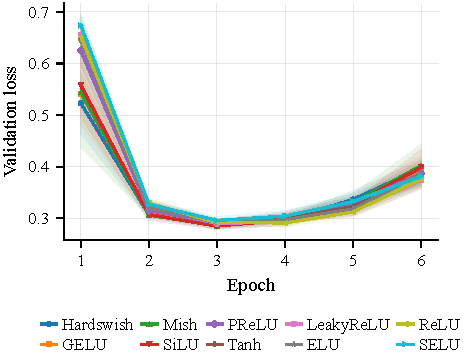
\includegraphics[width=0.92\columnwidth]{assets/convergence_curves.pdf}
  \caption{Validation loss for BiGRU+GRU with the same
  activation in both dense layers. Each line shows a five-seed
  mean; shading shows $\pm1$ SD. Only epochs reached by all
  five runs are shown.}
  \label{fig:convergence_curves}
\end{figure}

\subsection{Variation Between Runs}
\label{sec:seed_variation}

GRU configurations have lower median accuracy SDs in both
architectures (Table~\ref{tab:sweep_summary}). Pooling the
200 configuration SDs within each family gives medians of
0.30 percentage points for GRU and 0.50 for LSTM, about
\textbf{40\% lower} for GRU.

All eight configurations with an SD above one point use
LSTM. Hardswish + LeakyReLU in BiLSTM+LSTM has the largest
SD (9.27 points) and a mean of 82.06\%, below the plotted
range in Fig.~\ref{fig:architecture_spread}. Its five runs
range from 65.50\% to 86.85\%, including the lowest accuracy
among all 2{,}000 runs. This wide range shows why a
configuration's mean alone does not describe its consistency.

For each configuration, we also compare precision and recall
after averaging each metric across five seeds. The largest
absolute gap is 6.89 percentage points, compared with 24.17
points for individual runs. Averaging can therefore hide larger gaps in individual runs.

The reported mean training time is 13.4~s per run on an
NVIDIA RTX 5080. BiGRU+GRU has about 734K parameters,
compared with 764K for BiLSTM+LSTM
(Table~\ref{tab:architectures}).

\FloatBarrier

\section{Discussion}
\label{sec:discussion}

\subsection{RQ1: How much accuracy variation comes from architecture, activation choice and training seeds?}
\label{sec:rq1}

Seed variation accounts for 58.7\% of total variance,
architecture for 26.7\%, the architecture--activation
interaction for 10.9\%, and activation pairs for 3.7\%
(Table~\ref{tab:variance}). Seed variation is the largest
component in this setting.

\subsection{RQ2: Which architectures achieve higher mean test accuracy?}
\label{sec:rq2}

Both GRU architectures have higher mean test accuracy than
both LSTM architectures (Table~\ref{tab:sweep_summary}).
The family mean gap is 0.79 percentage points, while making
the second recurrent layer bidirectional changes mean
accuracy little.

\subsection{RQ3: How do accuracy gaps between leading activation pairs compare with variation across seeds?}
\label{sec:rq3}

Among the leading configurations, mean accuracy gaps are
small relative to seed SDs (Table~\ref{tab:top_configs}).
These results do not establish a consistently best pair,
but they also do not establish that all pairs perform equally.

\subsection{RQ4: Do single-run rankings agree with five-seed rankings?}
\label{sec:rq4}

The single-run and five-seed rankings show little agreement
(Table~\ref{tab:reproducibility}). A high rank from one run
therefore does not reliably identify the pairs with the
highest means after repeated training.

\subsection{RQ5: How does activation choice affect early learning?}
\label{sec:rq5}

Activation choice affects epoch-one validation accuracy
(Section~\ref{sec:learning}), while validation losses become
closely grouped by epoch three
(Fig.~\ref{fig:convergence_curves}). The early differences
do not establish an advantage in final test accuracy.

\subsection{RQ6: Which architectures give more consistent test accuracy across training runs?}
\label{sec:rq6}

GRU configurations show lower variation across seeds
(Table~\ref{tab:sweep_summary}). Their pooled median SD is
0.30 percentage points, compared with 0.50 for LSTM,
about 40\% lower. All eight configurations with an SD
above one point use LSTM (Section~\ref{sec:seed_variation}).

\subsection{Limitations}

The study uses one dataset and a fixed data split. It does
not measure variation caused by changing the split or
establish whether the activation patterns hold on other
datasets. 

\section{Conclusion}

This study examines how architecture, dense-layer activation
choice and training seeds affect sentiment-classification
accuracy on IMDb. We evaluate 100 ordered activation pairs
across four recurrent architectures, with five seeds per
configuration, giving 2{,}000 runs. This design allows us to
compare differences between configurations with the variation
observed when the same configuration is trained repeatedly.
Seed variation accounts for 58.7\% of total test-accuracy
variance, architecture for 26.7\%, activation pairs for 3.7\%,
and their interaction for 10.9\% (Table~\ref{tab:variance}).

Architecture choice shows a clearer pattern than the ordering
of individual activation pairs. GRU exceeds LSTM by 0.79
percentage points in family mean accuracy
(Table~\ref{tab:sweep_summary}). GRU configurations also have
about 40\% lower median SD across seeds, while all eight
configurations with an SD above one point use LSTM
(Section~\ref{sec:seed_variation}). Thus, under the tested
settings, GRU combines higher average accuracy with greater
consistency across training runs.

The evidence for preferring a particular activation pair is
less clear. Single-run rankings show little agreement with
five-seed rankings (Table~\ref{tab:reproducibility}), and
accuracy gaps among the leading pairs are small relative to
their seed SDs (Table~\ref{tab:top_configs}). These findings
limit what a single high score can tell us about which pair
will perform well across repeated training. They do not show
that all activation pairs perform equally. Activation choice
also affects early learning, although validation losses become
closely grouped by epoch three
(Fig.~\ref{fig:convergence_curves}).

The main practical finding is that activation comparisons
should report both mean accuracy and variation across training
seeds. In this study, architecture choice has a larger effect
on accuracy than activation-pair choice, while repeated runs
change which pairs appear strongest. 
{\footnotesize
\begin{thebibliography}{23}
\setlength{\itemsep}{-2.2pt}

% -- Gated Recurrent Architectures --

\bibitem{hochreiter1997}
S. Hochreiter and J. Schmidhuber,
``Long short-term memory,''
\textit{Neural Computation}, vol.~9, no.~8, pp.~1735--1780, Nov. 1997.

\bibitem{cho2014}
K. Cho, B. van Merri\"{e}nboer, C. Gulcehre, D. Bahdanau, F. Bougares,
H. Schwenk, and Y. Bengio,
``Learning phrase representations using RNN encoder-decoder for statistical
machine translation,''
in \textit{Proc. EMNLP}, 2014, pp.~1724--1734.

\bibitem{chung2014}
J. Chung, C. Gulcehre, K. Cho, and Y. Bengio,
``Empirical evaluation of gated recurrent neural networks on sequence
modeling,''
\textit{arXiv preprint arXiv:1412.3555}, 2014.

\bibitem{schuster1997}
M. Schuster and K.~K. Paliwal,
``Bidirectional recurrent neural networks,''
\textit{IEEE Trans. Signal Process.}, vol.~45, no.~11,
pp.~2673--2681, Nov. 1997.

% -- Activation Functions --

\bibitem{nair2010}
V. Nair and G.~E. Hinton,
``Rectified linear units improve restricted Boltzmann machines,''
in \textit{Proc. ICML}, 2010, pp.~807--814.

\bibitem{maas2013}
A.~L. Maas, A.~Y. Hannun, and A.~Y. Ng,
``Rectifier nonlinearities improve neural network acoustic models,''
in \textit{Proc. ICML Workshop on Deep Learning for Audio, Speech and
Language Processing}, 2013.

\bibitem{he2015}
K. He, X. Zhang, S. Ren, and J. Sun,
``Delving deep into rectifiers: Surpassing human-level performance on
ImageNet classification,''
in \textit{Proc. ICCV}, 2015, pp.~1026--1034.

\bibitem{clevert2015}
D. Clevert, T. Unterthiner, and S. Hochreiter,
``Fast and accurate deep network learning by exponential linear units
(ELUs),''
\textit{arXiv preprint arXiv:1511.07289}, 2015.

\bibitem{klambauer2017}
G. Klambauer, T. Unterthiner, A. Mayr, and S. Hochreiter,
``Self-normalizing neural networks,''
in \textit{Proc. NeurIPS}, 2017, pp.~971--980.

\bibitem{hendrycks2016}
D. Hendrycks and K. Gimpel,
``Gaussian error linear units (GELUs),''
\textit{arXiv preprint arXiv:1606.08415}, 2016.

\bibitem{ramachandran2017}
P. Ramachandran, B. Zoph, and Q.~V. Le,
``Searching for activation functions,''
\textit{arXiv preprint arXiv:1710.05941}, 2017.

\bibitem{misra2020}
D. Misra,
``Mish: A self regularized non-monotonic activation function,''
in \textit{Proc. BMVC}, 2020.

\bibitem{howard2019}
A. Howard \textit{et al.},
``Searching for MobileNetV3,''
in \textit{Proc. ICCV}, 2019, pp.~1314--1324.

\bibitem{apicella2021}
A. Apicella, F. Donnarumma, F. Isgr\`{o}, and R. Prevete,
``A survey on modern trainable activation functions,''
\textit{Neural Networks}, vol.~138, pp.~14--32, 2021.

\bibitem{nwankpa2018}
C. Nwankpa, W. Ijomah, A. Gachagan, and S. Marshall,
``Activation functions: Comparison of trends in practice and research for
deep learning,''
\textit{arXiv preprint arXiv:1811.03378}, 2018.

% -- Sentiment Analysis --

\bibitem{maas2011}
A.~L. Maas, R.~E. Daly, P.~T. Pham, D. Huang, A.~Y. Ng, and C. Potts,
``Learning word vectors for sentiment analysis,''
in \textit{Proc. ACL}, 2011, pp.~142--150.

\bibitem{ahmed2025}
S.~A. Ahmed \textit{et al.},
``Comparative analysis of activation functions in LSTM models for sentiment
classification,''
\textit{IJARCCE}, vol.~14, no.~4, Apr. 2025.

\bibitem{zhu2022}
Y. Zhu and R. Tan,
``A novel activation function based recurrent neural networks and their
applications on sentiment classification and log anomaly detection,''
\textit{Frontiers in Neurorobotics}, vol.~16, 2022.

\bibitem{socher2013}
R. Socher, A. Perelygin, J. Wu, J. Chuang, C.~D. Manning, A. Ng,
and C. Potts,
``Recursive deep models for semantic compositionality over a sentiment
treebank,''
in \textit{Proc. EMNLP}, 2013, pp.~1631--1642.

\bibitem{tang2015}
D. Tang, B. Qin, and T. Liu,
``Document modeling with gated recurrent neural network for sentiment
classification,''
in \textit{Proc. EMNLP}, 2015, pp.~1422--1432.

% -- Direct Competitors --

\bibitem{eger2018}
S. Eger, P. Youssef, and I. Gurevych,
``Is it time to swish? Comparing deep learning activation functions across
NLP tasks,''
in \textit{Proc. EMNLP}, 2018, pp.~4423--4433.

\bibitem{farzad2019}
A. Farzad, H. Mashayekhi, and H. Hassanpour,
``A comparative performance analysis of different activation functions in
LSTM networks for classification,''
\textit{Neural Computing and Applications}, vol.~31,
pp.~2507--2521, 2019.

\bibitem{essaiAli2022}
M.~H. Essai~Ali, A.~I. Taloba, M.~F. Farhan, and R.~A. Abozeid,
``Developing novel activation functions based deep learning LSTM for
classification,''
\textit{IEEE Access}, vol.~10, pp.~96578--96591, 2022.

\end{thebibliography}
}
\end{document}
